\section{\uppercase{Related Work}}
\label{sec:related}

\subsection{Image-Based Virtual Try-On}
Early try-on pipelines such as VITON~\cite{han2018viton} and VITON-HD~\cite{choi2021vitonhd} warp the garment onto the person and then blend it in with a generative adversarial network (GAN). More recent work replaces this approach with a latent diffusion model~\cite{rombach2022ldm} that is conditioned on the garment, for example LaDI-VTON~\cite{morelli2023ladivton} and StableVITON~\cite{kim2024stableviton}. The three models studied in this paper differ mostly in how they inject the garment into the denoising network. OOTDiffusion~\cite{xu2025ootdiffusion} encodes the garment with a distinct outfitting UNet and fuses its features into the self-attention layers of the denoising UNet. IDM-VTON~\cite{choi2024idmvton} leverages a pretrained diffusion model, SDXL~\cite{podell2024sdxl}, combined with a similar garment UNet (GarmentNet) for fine detail and an IP-Adapter~\cite{ye2023ipadapter} for high-level semantics. On the other hand, CatVTON~\cite{chong2025catvton} uses no extra encoder at all. The person and garment images are concatenated and processed by one inpainting UNet. Figure~\ref{fig:architectures} summarises these differences. All three works evaluate only the final image, with metrics such as FID, KID, SSIM and LPIPS. In contrast, we study how each model arrives at that image.

\begin{figure}[t]
  \centering
  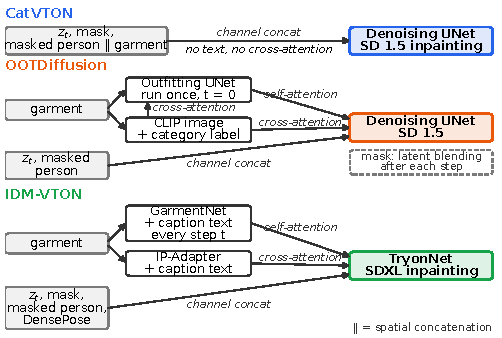
\includegraphics[width=\columnwidth]{figures/architectures.pdf}
  \caption{Inputs of the three models, with $z_t$ the noisy latent. \catvton places person and garment side by side ($\Vert$) in one inpainting UNet without text or cross-attention. \ootd and \idm encode the garment with a separate UNet whose features enter the self-attention layers. \ootd runs its outfitting UNet once before denoising, while \idm runs GarmentNet at every step. Through cross-attention, \ootd also receives the garment's CLIP image embedding with a category label, which is empty for the HD checkpoint used here. \idm receives an IP-Adapter embedding with a garment caption. \ootd uses the mask only to blend the latents after each step.}
  \label{fig:architectures}
\end{figure}


\subsection{Diffusion Models and Their Sampling Dynamics}
Diffusion models~\cite{ho2020ddpm} generate an image by gradually removing noise. With DDIM sampling~\cite{song2021ddim}, it is possible to sample them in fewer steps and to read out an estimate of the clean, final image at every step. Several works have observed that this process is coarse-to-fine, with high-noise steps responsible for coarse content and low-noise steps for detail~\cite{choi2022p2}. Since adding noise affects the high frequencies of natural images first~\cite{rissanen2023ihdm,dieleman2024spectral}, diffusion can also be seen as a frequency-ordered generation. High-level features, in turn, can be edited in the bottleneck of the UNet during the earlier steps~\cite{kwon2023hspace}. These studies concern unconditional or text-conditioned generation. In virtual try-on, however, the model is conditioned on a garment image which already contains all of the fine detail. Thus, it is not obvious that the same order holds. 

\subsection{Analysing Intermediate Predictions}
Usually, intermediate steps are used for editing rather than for analysis. Examples include SDEdit~\cite{meng2022sdedit}, which re-noises an image to an intermediate step before denoising it again and Prompt-to-Prompt~\cite{hertz2023p2p}, which injects attention maps during a chosen part of the trajectory. Both works rely on the intuition that different properties are decided at different steps. This method has also been applied in virtual try-on by LPH-VTON~\cite{liu2026lphvton} using latent hand-over from a structure-biased to a texture-biased model partway through denoising. To our knowledge, no prior work measures when the individual garment properties settle in different try-on models, which is what we address in this paper.

